\subsection{RAID 0}

RAID 0 es una técnica de almacenamiento cuyo objetivo principal es aumentar el rendimiento, no la confiabilidad.

Conceptualmente, RAID 0 divide la información en bloques y distribuye esos bloques entre dos o más discos. En lugar de escribir un archivo completo en un único disco, los bloques se reparten de forma alternada.

Por ejemplo, si un archivo se divide en diez bloques, se reparten entre dos discos como se muestra en la figura \ref{fig:raid0}.

\begin{figure}[!ht]
  \centering
  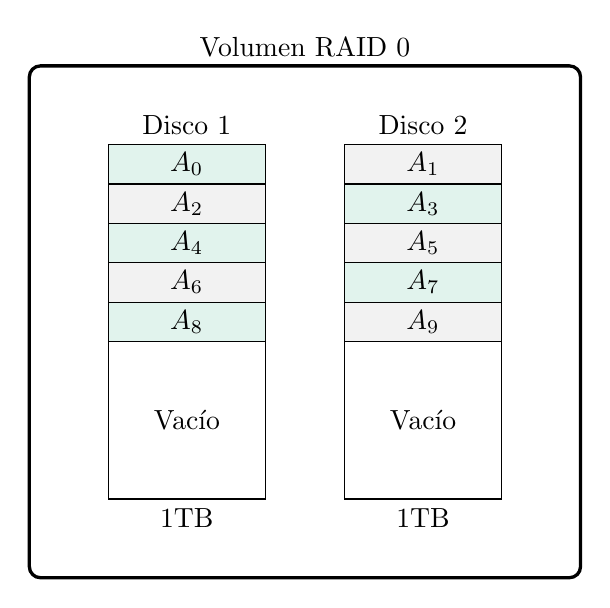
\begin{tikzpicture}
    \node[above] at (1,2.5) {Disco 1};
    \foreach \y\t\c in {
        0/8/white!95!blue!93!green,
        0.5/6/gray!10,
        1/4/white!95!blue!93!green,
        1.5/2/gray!10,
        2/0/white!95!blue!93!green}{
      \draw[fill=\c] (0,\y) rectangle node{\(A_\t\)} (2,{0.5+\y});
    }
    \draw (0,0) rectangle node{Vacío} (2,-2);
    \node[below] at (1,-2) {1TB};

    \node[above] at (4,2.5) {Disco 2};
    \foreach \y\t\c in {
        0/9/gray!10,
        0.5/7/white!95!blue!93!green,
        1/5/gray!10,
        1.5/3/white!95!blue!93!green,
        2/1/gray!10}{
      \draw[fill=\c] (3,\y) rectangle node{\(A_\t\)} (5,{0.5+\y});
    }
    \draw (3,0) rectangle node{Vacío} (5,-2);
    \node[below] at (4,-2) {1TB};

    \draw[very thick,rounded corners] (-1,-3) rectangle (6,3.5);
    \node[above] at (2.5,3.5) {Volumen RAID 0};
  \end{tikzpicture}
  \caption{Tamaño del volumen de RAID 0: 2TB.}
  \label{fig:raid0}
\end{figure}

Cuando se lee o escribe el archivo, ambos discos trabajan simultáneamente. Esto permite que la velocidad de transferencia sea considerablemente mayor que la de un solo disco, ya que las operaciones se realizan en paralelo.

\paragraph{Ventajas:}
\begin{itemize}
  \item Mayor velocidad de lectura y escritura.
  \item Se aprovecha el 100\% de la capacidad total de los discos.
  \item Implementación sencilla.
\end{itemize}

\paragraph{Desventajas:}
\begin{itemize}
  \item No proporciona redundancia ni tolerancia a fallos.
  \item Si falla un solo disco, se pierde toda la información del arreglo, porque cada archivo está repartido entre todos los discos.
\end{itemize}

\paragraph{Ejemplo}
Si se tienen dos discos de 1 TB, la capacidad total disponible es de 2 TB. Pero si uno de los discos deja de funcionar, el sistema pierde todos los archivos, ya que faltan partes de cada uno de ellos.

\begin{table}[!ht]
  \centering
  \begin{tabular}{l|c}
    Cantidad de discos mínima & 2 \\\hline
    Cantidad de discos que pueden fallar & 0 \\ \hline
    Velocidad de escritura relativa a un disco & \(N\times\)VDisco~[MB/s] \\\hline
    Velocidad de escritura ponderada & 10 \\ \hline
    Velocidad de lectura relativa a un disco & \(N\times\)VDisco~[MB/s] \\ \hline
    Velocidad de lectura ponderada & 10 \\ \hline
    Costo & Bajo
  \end{tabular}
  \caption{Características del RAID 0.}
\end{table}
